\section{Les classes \enquote{agents}}
\subsubsection{Sprints 1 et 2}
Lors du premier sprint, nous avons commencer par mettre en place la base du programme. Nous avions prévu de faire l'UML~\ref{v0.1}.

 Pour le modèle, il s'agissait de créer les classes :
\begin{itemize}
\item Turtle, qui représente une tortue~;
\item Point, pour stocker les coordonnées d'une tortue~;
\item Line, qui est composé de points, et qui permet aux tortues de laisser une trace (instruction pendown)~;
\item World.
\end{itemize}


\begin{figure}[h]
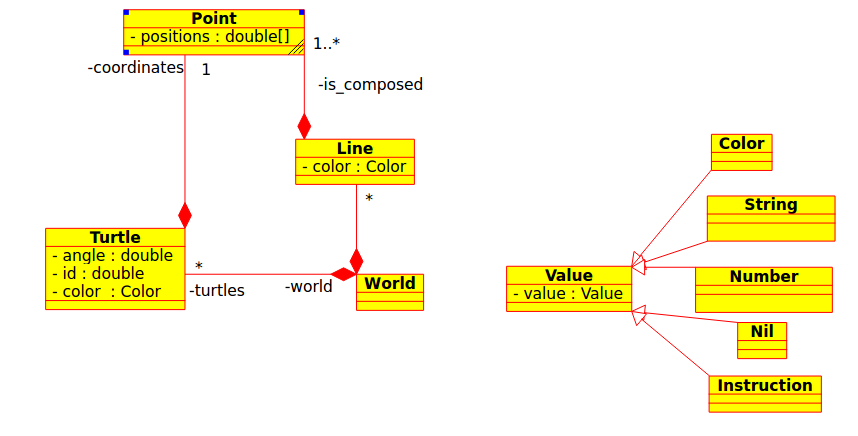
\includegraphics[scale=0.5]{doc/report/uml/v01.png}
\caption{\label{v0.1} UML de la version 0.1 prévue}
\end{figure}


La classe World représente le monde des tortues. Il contient la liste des tortues, et les lignes tracées par ces tortues car c'est lui qui communique avec l'interface pour l'affichage de ces lignes.
A la fin du sprint 1, on pouvait voir une tortue avancer et tracer une ligne sur son passage.
Nous avions réalisé le schéma~\ref{v0.1R}. Il respecte la version prévue, en dehors de la classe Instruction, qui n'était finalement pas nécessaire. Les instructions sont des mot-clés du langage.\\

Pour le second sprint, nous avons ajouté une classe Agent, super classe de World, Turtle et Zone. En effet, elles sont toutes les trois des agents, et ont donc des comportements similaires (cf ~\ref{v0.2}).

Ces classes ont chacun un parent, l'agent qui l'a créer, une liste d'enfants, et des propriétés. Les propriétés sont des variables définit par l'utilisateur lors de la définition du code de l'agent, donc surtout utile pour les tortues.

Le monde a une taille,et deux listes de d'espèce de tortues (dit \enquote{breed}) : les espèces nommées et les anonymes, qui sont des \enquote{turtles} dans le code.

Comme le montre ce code, on peut créer des tortues nommées ou pas. Une tortue anonyme s'écrit \enquote{new agent} et une nommée \enquote{agent listener}, listener étant le nom choisi par l'utilisateur.

\begin{lstlisting}[language=Stibbons]
agent listener () {
	fd 2
}

new listener ()

new agent {
	lt 30
	fd 5
}
\end{lstlisting}
\subsubsection{Sprints 3 et 4}
Lors du troisième sprint, nous avons mis en place des pointers intelligents dans toutes nos classes (cf figure~\ref{v0.3}). Le but de ce sprint était la mise en place de la communication entre les agents. Les tortues peuvent communiquer avec les zones par écriture dans leurs propriétés. Les tortues peuvent communiquer entre elles grâce à des méthodes comme sendAll(message), recv(), etc.

L'étape suivante était d'ajouter des fonctionnalités tel que la maîtrise du temps et l'exportation du modèle. Ces ajouts ne provoquent pas de changement du coté du modèle, si ce n'est quelques méthodes dans les classes World et Turtle et Zone pour l'exportation du modèle.

L'exportation du modèle consiste à créer une sauvegarde de l'état du modèle à un instant t dans un fichier JSON grâce à la bibliothèque JSON Spirit.
Cela permettra ensuite, en passant par une transformation en CSV, d'avoir un tableau avec toutes ces données, ce qui offre la possibilité d'avoir des diagrammes de l'évolution du monde.

La maîtrise du temps se fait grâce à un bouton pause, qui arrête les threads qui s'exécutent, ou par un slider qui permet de ralentir ou de diminuer la vitesse. Cela se fait dans le code grâce à une méthode sleepfor() qui prend en paramètre un temps donné. Cette fonctionnalité n'impact pas le modèle.

\section{Les types}
\subsubsection{Sprints 1 et 2}
Lors du premier sprint, nous mettions en place certains types Stibbons, comme Color, pour la couleur, ou Nil qui a une valeur nulle. Ils héritent de Value, une classe abstraite qui contient une valeur et ses accesseurs.
Les instructions tel que pendown, forward, etc., sont finalement des mots clés dans la grammaire du langage, et non pas des instructions, contrairement à ce que nous avions prévu (cf UML~\ref{v0.1}).
Elles sont définis dans le modèle dans la classe Turtle (cf UML~\ref{v0.2}).

\begin{figure}[h]
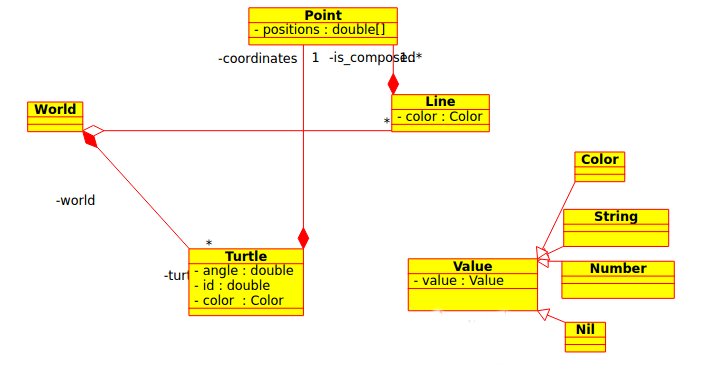
\includegraphics[scale=0.5]{doc/report/uml/v01reel.png}
\caption{\label{v0.1R} UML de la version 0.1 réalisée}
\end{figure}

Lors du sprint deux, les types Stibbons sont les mêmes, mais leurs définitions s'est un peu compléxifiées en passant par une classe Simple-value, pour la mise en place des mutexs. Une énumeration des types Stibbons existe, elle est utilisée avec la méthode getType() pour pouvoir connaître le type de Value.
Pour que l'utilisateur puisse écrire des fonctions dans le code, nous avons ajouté une classe Function, qui stocke un arbre, qui contient le code la fonction, déjà parsé.
\\ Des mutexs ont été ajouté dans toutes les classes pour assurer que les threads sont thread-safe (cf figure~\ref{v0.2}).

\begin{figure}[h]
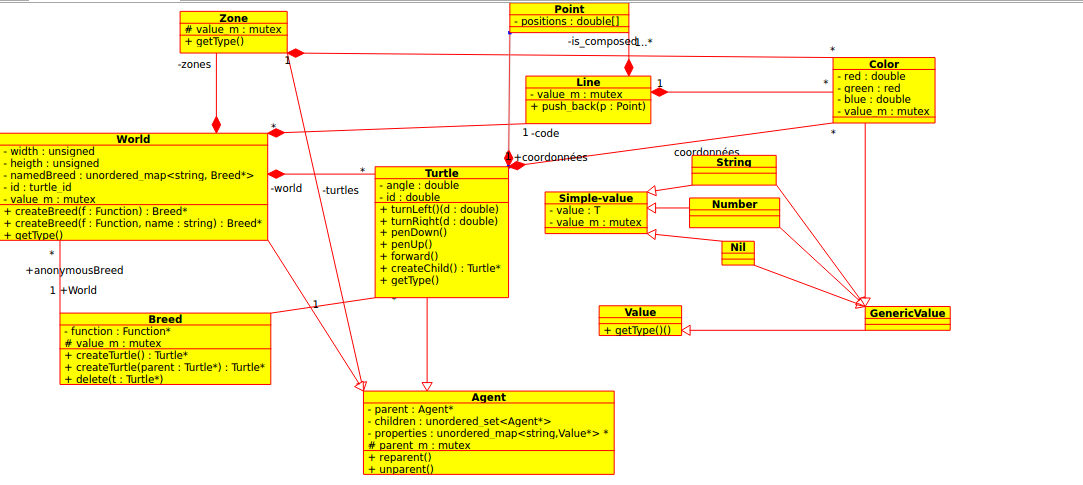
\includegraphics[scale=0.45]{doc/report/uml/v02.png}
\caption{\label{v0.2} UML version 0.2}
\end{figure}
\subsubsection{Sprints 3 et 4}
Lors du troisième sprint, nous avons ajouté une sous-classe de Function : userFunction, qui représentent les fonctions crées par l'utilisateur (cf figure~\ref{v0.3}) . Nous avons également créer des fonctions standarts comme ask-zone, qui permet de donner un ordre aux zones.
\begin{figure}[h]
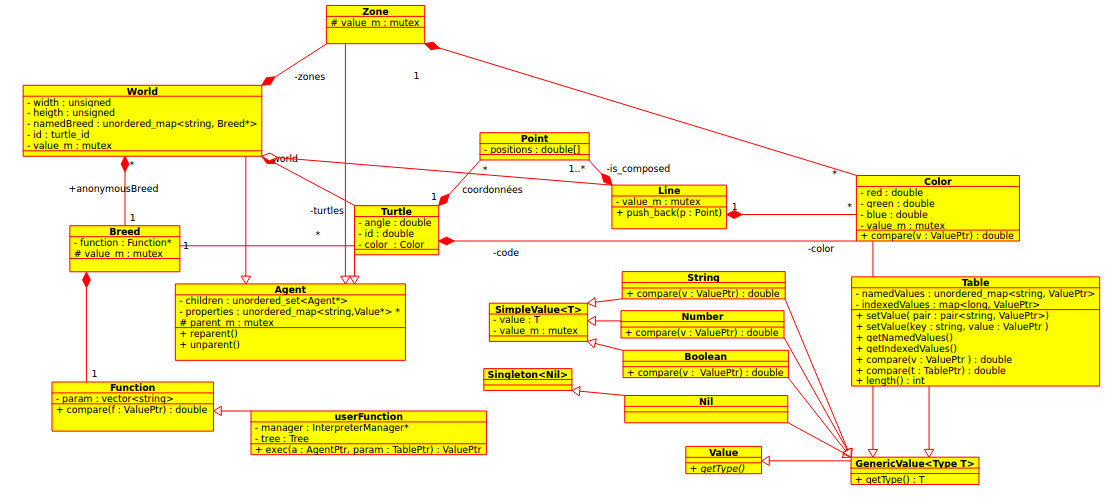
\includegraphics[scale=0.4]{doc/report/uml/v03.png}
\caption{\label{v0.3} UML version 0.3}
\end{figure}

On les différencie des instructions par leurs parenthéses derrière leur nom.
L'ajout de table fait aussi partit de ce sprint. Nous avons choisi, pour notre langage un seul type de conteneur : les tableaux.
Nous les écrivons façon php, avec des accolades.
\begin{lstlisting}
a = 12

t = {18,red,"bla"}
v = { "bla" : "blou", "blue" : blue, a : 29 }

println(t[2])
t[2] = 32
println(t[2])
v[] = 48
println(v)

u = 5 new agent {
	while true fd 20
}
\end{lstlisting}

Nous avons mis en place des mutexs récursifs lors du sprint quatre. Ils permettent à un thread de verrouiller plusieurs fois la même ressources alors qu'elle est déjà verrouillée. C'est la seule différence avec le mutex normal. 

Ces mutexs permettent d'éviter des blocages dans certaines situations (fonctions récursives, ...) .
L'UML~\ref{v0.4} est l'état final du modèle car le sprint 5 n'y a apporté aucune modification.
\begin{figure}[h]
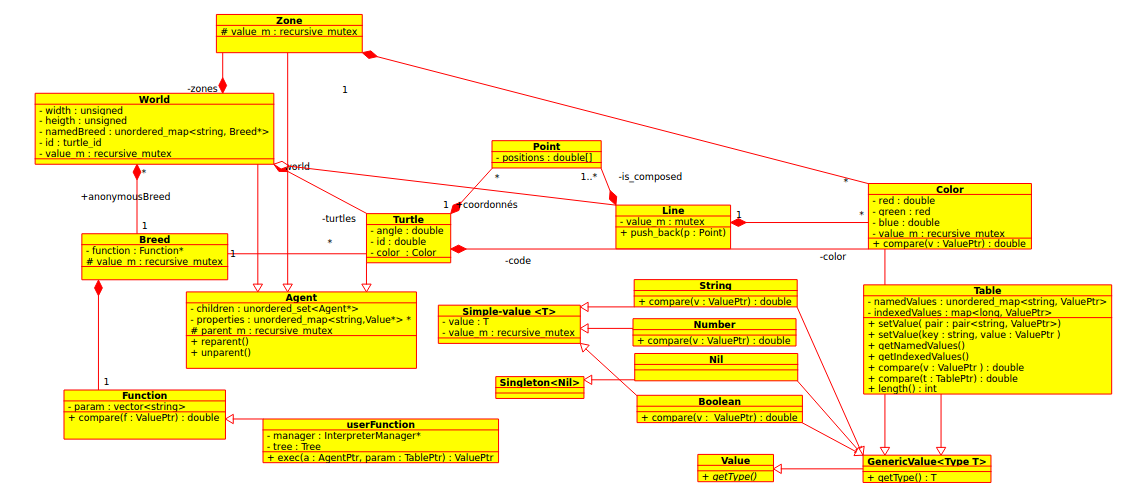
\includegraphics[scale=0.4]{doc/report/uml/v04.png}
\caption{\label{v0.4} UML version 0.4}
\end{figure}

